%------------------------------------------------------------------------------------
%	CHAPTER 2
%------------------------------------------------------------------------------------
\chapterimage{headerCap.jpeg}
\chapter{União com C++}

\begin{remark}
	Você não é Assembly mas eu quebro muito a cabeça para te entender. (Davyd Maker) 
\end{remark}

\section{Porquê fazer isso?}\index{União com C++}
Talvez a pergunta mais simples seja: O que ganhamos com isso? Fico pensando sinceramente se vale a pena essa união do C++ com o Assembly e a resposta é sempre sim, isso deu muito certo com o ambiente embarcado das placas Arduino e porquê não daria conosco? É verdade que todo casamento tem seus problemas, mas se fosse tudo uma lua-de-mel seria bem esquisito.

Praticamente gosto de utilizar o C++ para realizar as entradas e saídas de dados enquanto que o Assembly toda a parte de processamento. Vejamos como isso funciona e alguns exemplos nas seções seguintes.

\section{Programa 5 - Troca de Informações}\index{União com C++}

Diferentemente do que sempre fazemos vamos começar iniciando um programa em C++, chamaremos de "troca.cpp" com o seguinte conteúdo:
\begin{lstlisting}[]
# include <iostream>

using namespace std;

extern "C" int GetValorASM(int a);

int main() {
	cout<<"ASM me deu "<<GetValorASM(32)<<endl;
	return 0;
}
\end{lstlisting}

O comando \textbf{include} indica que iremos trabalhar com uma entrada de dados e a instrução "\textit{using namespace std;}" serve para definir um "espaço para nomes". Isso permite a definição de estruturas, classes e constantes que estão vinculadas para definir funções da biblioteca padrão. 

A instrução que realmente nos interessa é a "extern" que indica o nome de uma função que devemos definir, essa recebe um argumento inteiro e retorna também outro. Em linguagens de alto nível sempre temos um método de entrada neste caso é o "\textbf{int main()}", neste damos uma saída em cadeia de caracteres para o terminal informando: "ASM me deu " + retorno da função \textit{GetValorASM} quando esta recebe 32.

\subsection{Agora sim vamos para o Assembly}\index{União com C++}
Gostaria muito que não se assustasse com o tamanho do programa, pois o mesmo é extremamente pequeno (pensou que ia falar grande?), mas nesse começo quero deixar as coisas simples, crie um programa chamado "troca.asm" e insira a seguinte codificação:
\begin{lstlisting}[]
section .text

global GetValorASM

GetValorASM:
	mov eax, edi
	add eax, 1
	ret	
\end{lstlisting}

Acredito que nem precise explicar, mas vamos assim mesmo. Antes vamos entender seu fluxo:
\begin{figure}[H]
	\centering
	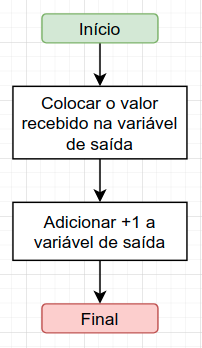
\includegraphics[width=0.25\textwidth]{Pictures/cap02/programa5}
	\caption{Fluxograma do Programa \textbf{Troca de Informações}}
\end{figure}

Primeiro definimos a parte de entrada, não precisamos da sessão .data então vamos direto para a .text porém com uma grande mudança ao invés de definirmos uma "\textit{\_start}" vamos chamar um método que o programa C++ está esperando e o definiu "\textit{GetValorASM}" (atenção com as letras é tudo case-sensitivo aqui!). 

Nesta função pegamos o valor do registrador \textbf{EDI} (que é utilizado para a passagem do primeiro parâmetro). Outros registradores utilizados são \textbf{ESI} para o segundo e \textbf{EDX} para o terceiro. Colocamos o valor de \textbf{EDI} em \textbf{EAX} (que é utilizado como valor de retorno do método - SEMPRE) e a este adicionamos mais um, ou seja o valor de retorno será sempre o valor de entrada mais um.

\subsection{Modificar o arquivo makefile}\index{União com C++}
Como agora estamos trabalhando com o C++ precisamos realizar uma pequena alteração para o linkeditor, não podemos mais utilizar o \textbf{LD} e devemos passar a utilizar o \textbf{G++}, assim nossa nova codificação para este deve ter o comando: \\
{\ttfamily\$ g++ troca.o troca.cpp -o troca}

Ou seja nosso arquivo agora terá a seguinte codificação:
\begin{lstlisting}[]
NOME = troca

all: $(NOME).cpp $(NOME).o
	g++ $(NOME).o $(NOME).cpp -o $(NOME)
	rm -rf $(NOME).o

%.o: %.asm
	nasm -f elf64 $<	
\end{lstlisting}

Continuamos utilizando o comando \textbf{make} para compilar e linkeditar sem o menor problema e ao executarmos a instrução {\ttfamily ./troca}, teremos como resposta: \\
{\ttfamily\$ ASM me deu 33}

Realmente as coisas estão começando a ficar fáceis demais, e me falaram que o Assembly era difícil.

% Final do Capítulo
\clearpage